\documentclass[border=3pt,tikz]{standalone}

\usepackage{minkowski}

\begin{document}
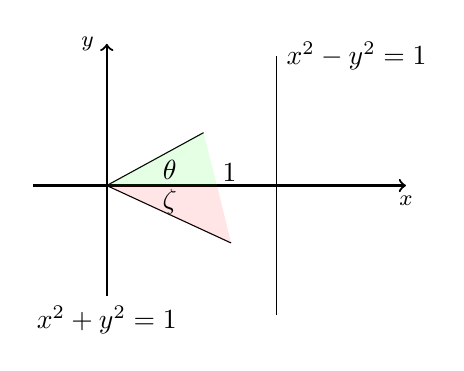
\begin{tikzpicture}[scale=2.0]

    \def\xrange{1.4}

    \coordinate (O) at (0,0);
    \coordinate (T) at (0,\xrange+0.2);

    \coordinate (A) at ({0.7*cosh(0.5)},{-0.7*sinh(0.5)});
    \coordinate (B) at ({0.7*cos(0.5 r)},{0.7*sin(0.5 r)});
    \coordinate (C) at (0, 0.96);

    % AXES
    \draw[->,thick] (0,-\xrange/2) -- (0,\xrange/2+0.2) node[left=1] {\footnotesize $y$};
    \draw[->,thick] (-\xrange/3,0) -- (\xrange+0.5,0) node[below=0] {\footnotesize $x$};

    \draw[black,samples=\Nsamples,smooth,variable=\x,domain=90:-90] plot({(0.7*cos(\x))},{(0.7*sin(\x))}) node[below] {$x^2 + y^2 = 1$};
    \draw[black,samples=\Nsamples,smooth,variable=\x,domain=-1:1] plot({(0.7*cosh(\x))},{(0.7*sinh(\x))}) node[right] {$x^2 - y^2 = 1$};

    \draw[black] (O) -- (A) node at (0.78,0.08) {$1$};
    %\draw[red,samples=\Nsamples,smooth,variable=\x,domain=-0.5:0] plot({(0.7*cosh(\x))},{(0.7*sinh(\x))});
    \fill[red,opacity=0.1,thick,samples=\Nsamples,smooth,variable=\x,domain=-0.5:0] plot({(0.7*cosh(\x))},{(0.7*sinh(\x))}) -- (O) node[opacity=1,text=black] at (0.4,-0.1) {$\zeta$};
    \draw[black] (O) -- (B);
    \fill[green,opacity=0.1,thick,samples=\Nsamples,smooth,variable=\x,domain=0:0.5 r] plot({(0.7*cos(\x))},{(0.7*sin(\x))}) -- (O) node[opacity=1,text=black] at (0.4,0.1) {$\theta$};

\end{tikzpicture}
\end{document}
